%\VignetteIndexEntry{The hts Package}
%\VignetteDepends{forecast}
%\VignetteKeywords{Hierarchical and grouped time series}
%\VignettePackage{hts}

\documentclass[nojss]{jss}
\usepackage{amsmath,graphicx,microtype,bm,tikz,tabulary,booktabs,mathtools,fancyvrb}
\mathtoolsset{showonlyrefs}
\usepackage[utf8]{inputenc} 
\fvset{samepage=true,frame=single}
\newcommand{\R}{\proglang{R}}

%% Change the default page sizes.
\usepackage[a4paper,text={16cm,24cm},centering]{geometry}
\raggedbottom

%\setlength{\topmargin}{-0.25in}
%\setlength{\textheight}{8.5in}
%\setlength{\oddsidemargin}{.0in}
%\setlength{\evensidemargin}{.0in}
%\setlength{\textwidth}{6.5in}
%\setlength{\footskip}{.5in}

\def\pred#1#2#3{#1_{\text{#2},#3}}
\def\y#1#2{\pred{y}{#1}{#2}}
\def\yhat#1#2{\hat{y}_{\text{#1},#2}}
\def\ytilde#1#2{\tilde{y}_{\text{#1},#2}}
\def\Shat#1#2#3{\hat{S}_{\text{#1},#2}^{(#3)}}

%% need no \usepackage{Sweave.sty}
  
\author{Rob J Hyndman, George Athanasopoulos, Han Lin Shang}
  
\title{\pkg{hts}: An {\R} Package for Forecasting Hierarchical or Grouped Time Series}
  
\Plainauthor{Rob Hyndman, George Athanasopoulos, Han Lin Shang}
  
\Plaintitle{The hts Package}
  
\Abstract{
This paper describes several methods that are currently available in the \pkg{hts} package, for forecasting hierarchical time series. The methods included are: top-down, buttom-up, middle-out and optimal combination. The implementation of these methods is illustrated by using regional infant mortality counts in Australia.
}
  
\Keywords{
top-down, bottom-up, middle-out, optimal combination
}

\Plainkeywords{
top-down, bottom-up, middle-out, optimal combination
}

\Address{
Rob Hyndman and George Athanasopoulos \\
Department of Econometrics \& Business Statistics\\
Monash University \\
Melbourne, Australia, VIC, 3800 \\
Email: \email{Rob.Hyndman@monash.edu} and 
\email{George.Athanasopoulos@monash.edu}
\vspace{.2in}

Han Lin Shang \\
ESRC Centre for Population Change\\
University of Southampton \\
Southampton, UK, SO17 1BJ \\
E-mail: \email{H.Shang@soton.ac.uk} \\
}


\begin{document}


%% For graphics
%% <<fig=TRUE,eval=TRUE, height=, width=>>=
    
\section*{Introduction}


Advances in data collection and storage have resulted in large numbers of time series that are hierarchical in structure, and clusters of which may be correlated. In many applications the related time series can be organized in a hierarchical structure based on dimensions such as gender, geography or product type. This has led to the problem of hierarchical time series modeling and forecasting. The aim of this article is to describe the {\R} functions that are available in the \pkg{hts} package \citep{HAH13}, for modeling and forecasting hierarchical and grouped time series.

Forecasting hierarchical time series has been the subject of increasing attention recently \citep[e.g.,][]{GAH09}, and has application in diverse fields. In macroeconomic forecasting, the national economic account is disaggregated into production, income and outlay, and capital transactions. Production is further classified into production in Britain and production in the rest of world; income and outlay and capital transactions are each further classified into persons, companies, public corporations, general government, and rest of world. In demographic forecasting, the mortality counts in Australia can be disaggregated by gender; within each gender, mortality counts can be further disaggregated by different states in Australia. The first example is referred to as a hierarchical time series, in which the order of disaggregation is unique. By contrast, the second example is a grouped time series, which can be thought of as hierarchical time series without a unique hierarchical structure. In other words, the order by which the series can be grouped is not unique --- the mortality counts in Australia can be first disaggregated by states and then by gender, or they can be disaggregated by gender first, and then by states.

Hierarchical forecasting methods allow the forecasts at each level to be summed giving the forecasts at the level above. When the data are grouped, the forecasts of each group must be equal to the forecasts of the individual series making up the group.
%, without any ad-hoc adjustment. Therefore, it has potential improvements in forecast accuracy, in comparison to the independent forecasts without adjustment \citep[e.g.,][]{FS90, ZT00, MSW03, Hubrich05}.

In the current statistical literature, existing approaches to hierarchical time-series forecasting usually involve either a top-down method or a bottom-up method or a combination of both methods often referred to as the ``middle-out'' approach. The top-down method involves forecasting the aggregated series, then disaggregating the forecasts based on the historical or forecast proportions \citep[see][for possible ways of choosing these proportions]{GS90,GAH09}. The bottom-up method involves forecasting each of the disaggregated series at the lowest level of the hierarchy, and then using aggregation to obtain forecasts at higher levels of the hierarchy \citep{Kahn98}. The middle-out method starts at an intermediate level of the hierarchy chosen by the user, and then aggregation is used to obtain forecasts at higher levels and disaggregation is used to obtain forecasts at lower levels. However, none of these methods takes the correlation among the series at each level into account. To address this issue, \cite{HAA+11} proposed a statistical method for optimal hierarchical forecasting.

This article proceeds as follows. Techniques for modeling and forecasting hierarchical time series are first reviewed and their implementations using the \pkg{hts} package are then described. Conclusions are given at the end.

\section*{Hierarchical forecasting methods}\label{sec:2}

\subsection*{Notation}

Figure~\ref{fig-9-4-hier} shows a $K=2$-level hierarchy. At the top of the hierarchy, level~0, is the ``Total'', the most aggregate level of the data. We denote as $y_t$ the $t$th observation of the ``Total'' series for $t=1,\dots,T$. Below this level we denote as $\y{j}{t}$ the $t$th observation of the series which corresponds to node $j$ of the hierarchical tree. The ``Total'' is disaggregated into two series at level~1 and each of these into three and two series respectively at the bottom level of the hierarchy (level~2). A denotes series~A at level~1; AB denotes series~B at level~2 within series~A at level~1, and so on.

The total number of series in a hierarchy is given by $n=1+n_1+\dots+n_K$ where $n_i$ is the number of series at level~$i$ of the hierarchy. In this case $n=1+2+5=8$.

\begin{figure}[!htb]
\caption{A two level hierarchical tree diagram}\label{fig-9-4-hier}
\centering
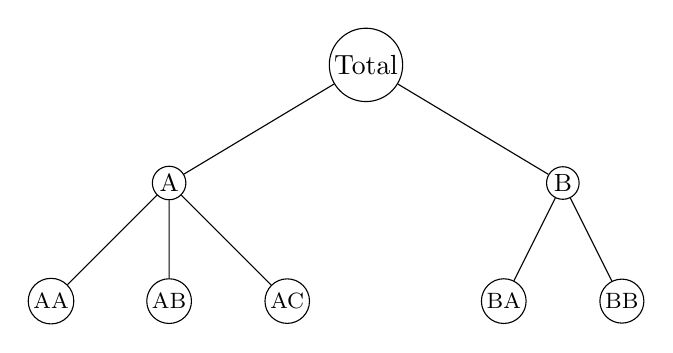
\begin{tikzpicture}
\tikzstyle{every node}=[circle,draw,inner sep=1pt]
\tikzstyle[level distance=.1cm]
\tikzstyle[sibling distance=.1cm]
%\tikzstyle{level 3}=[sibling distance=6.2mm,font=\tiny]
\tikzstyle{level 1}=[sibling distance=50mm,font=\small]
\tikzstyle{level 2}=[sibling distance=15mm,font=\footnotesize]

\node{Total}%[edge from parent fork down]
child {node {A}
       child {node {AA}}
       child {node {AB}}
       child {node {AC}}
}
child {node {B}
       child {node {BA}}
       child {node {BB}}
       %child {node {BC}}
};
\end{tikzpicture}
\end{figure}

For any time $t$, the observations of the bottom level series will aggregate to the observations of the series above. This can be effectively represented using matrix notation. We construct an $n\times n_K$ matrix referred to as the ``summing'' matrix $\bm{S}$ which dictates how the bottom level series are aggregated, consistent with the hierarchical structure. For the hierarchy in Figure \ref{fig-9-4-hier} we can write
\[
{\left[
  \begin{array}{c}
  y_{t} \\
  \y{A}{t} \\
  \y{B}{t} \\
  \y{AA}{t} \\
  \y{AB}{t} \\
  \y{AC}{t} \\
  \y{BA}{t} \\
  \y{BB}{t}
  \end{array}
  \right] }
=
{\left[\begin{array}{ccccc}
       1 & 1 & 1 & 1 & 1 \\
       1 & 1 & 1 & 0 & 0 \\
       0 & 0 & 0 & 1 & 1 \\
       1  & 0  & 0  & 0  & 0  \\
       0  & 1  & 0  & 0  & 0  \\
       0  & 0  & 1  & 0  & 0  \\
       0  & 0  & 0  & 1  & 0  \\
       0  & 0  & 0  & 0  & 1
       \end{array}
       \right] }
{\left[
  \begin{array}{c}
  \y{AA}{t} \\
  \y{AB}{t} \\
  \y{AC}{t} \\
  \y{BA}{t} \\
  \y{BB}{t}
  \end{array}
  \right]}
\]
or in more compact notation
\[
  \bm{y}_t=\bm{S}\bm{y}_{K,t},
\]
where $\bm{y}_t$ is a vector of all the observations in the hierarchy at time $t$, $\bm{S}$ is the summing matrix as defined above, and $\bm{y}_{K,t}$ is a vector of all the observation in the bottom level of the hierarchy at time $t$.

We are interested in generating forecasts for each series in the hierarchy. We denote as $\yhat{j}{h}$ the $h$-step-ahead forecast generated for the series at node $j$ having observed the time series up to observation $T$ and as $\hat{y}_{h}$ the $h$-step-ahead forecast generated for the ``Total'' series.\footnote{We have simplified the usual notation of $\hat{y}_{T+h|T}$ for brevity.} We refer to these as ``base'' forecasts. They are independent forecasts generated for each series in the hierarchy using a suitable forecasting method. These base forecasts are then combined to produce final forecasts for the whole hierarchy that aggregate in a manner that is consistent with the structure of the hierarchy. We refer to these as revised forecasts and denote them as $\ytilde{j}{h}$ and $\tilde{y}_{h}$ respectively.

There are a number of ways of combining the base forecasts in order to obtain revised forecasts. The following sections discuss some of the possible combining approaches.

\subsection*{Bottom-up method}

A commonly applied method for hierarchical forecasting is the bottom-up approach. This approach involves first generating base independent forecasts for each series at the bottom level of the hierarchy and then aggregating these upwards to produce revised forecasts for the whole hierarchy.

For example, for the hierarchy of Figure \ref{fig-9-4-hier} we first generate $h$-step-ahead base forecasts for the bottom level series: $\yhat{AA}{h}$, $\yhat{AB}{h}$, $\yhat{AC}{h}$, $\yhat{BA}{h}$ and $\yhat{BB}{h}$. Aggregating these up the hierarchy we get $h$-step-ahead forecasts for the rest of the series: $\ytilde{A}{h}= \yhat{AA}{h}+\yhat{AB}{h}+\yhat{AC}{h}$, $\ytilde{B}{h}= \yhat{BA}{h}+\yhat{BB}{h}$ and $\tilde{y}_{h}=\ytilde{A}{h}+\ytilde{B}{h}$. Note that for the bottom-up approach the revised forecasts for the bottom level series are equal to the base forecasts.

Using matrix notation we can again employ the summing matrix and write
\[
  \tilde{\bm{y}}_{h}=\bm{S}\hat{\bm{y}}_{K,h}.
\]
  
The greatest advantage of this approach is that no information is lost due to aggregation. On the other hand bottom level data can be quite noisy and more challenging to model and forecast \citep{SW79, STM88}.

\subsection*{Top-down method}

Top-down approaches involve first generating base forecasts for the ``Total'' series $y_t$ on the top of the hierarchy and then disaggregating these downwards. We let
$
  p_1,\ldots,p_{m_K}
$
be a set of proportions which dictate how the base forecasts of the ``Total'' series are to be distributed to revised forecasts for each series at the bottom level of the hierarchy. Once the bottom level forecasts have been generated we can use the summing matrix to generate forecasts for the rest of the series in the hierarchy. Note that for top-down approaches the top level revised forecasts are equal to the top level base forecasts, that is $\tilde{y}_{h}=\hat{y}_{h}$.

When the bottom-level series are noisy, the forecasts of the top-down approach can be more accurate than the bottom-up approach \citep{GG60, Fliedner99}. The performance of the top-down approach depends on three factors: (1)~the accuracy of the total series forecasts; (2)~the accuracy of the disaggregate proportions; (3)~the degree of accuracy in the base forecasts. \cite{GS90} studied the top-down approach extensively, and put forward 21 disaggregation methods. Furthermore, they found two promising methods that are also simple to use, namely average historical proportion and proportions of the historical averages.

\subsubsection{Average historical proportions }
The average historical proportions can be expressed as
\[
  p_j=\frac{1}{T}\sum_{t=1}^{T}\frac{y_{j,t}}{{y_t}}
\]
for $j=1,\dots,m_K$. Each proportion $p_j$ reflects the average of the historical proportions of the bottom level series $y_{j,t}$ over the period $t=1,\dots,T$ relative to the total aggregate $y_t$.

\subsubsection{Proportions of the historical averages}
The proportions of the historical averages are expressed by
$$
  p_j={\sum_{t=1}^{T}\frac{y_{j,t}}{T}}\Big/{\sum_{t=1}^{T}\frac{y_t}{T}}
$$
for $j=1,\dots,m_K$. Each proportion $p_j$ captures the average historical value of the bottom level series $y_{j,t}$ relative to the average value of the total aggregate $y_t$.

The greatest attribute of such top-down approaches is their simplicity to apply. One only needs to model and generate forecasts for the most aggregated top level series. In general these approaches seem to produce quite reliable forecasts for the aggregate levels and they are very useful with low count data. On the other hand, their greatest disadvantage is the loss of information due to aggregation. With these top-down approaches, we are unable to capture and take advantage of individual series characteristics such as time dynamics, special events, etc.

\subsubsection{Forecasted proportions}

An alternative approach that improves on the historical and static nature of the proportions specified above is to use forecasted proportions \citep{GAH09}.

To demonstrate the intuition of this method, consider a one level hierarchy. We first generate $h$-step-ahead base forecasts for all the series independently. At level~1 we calculate the proportion of each $h$-step-ahead base forecast to the aggregate of all the $h$-step-ahead base forecasts at this level. We refer to these as the forecasted proportions and we use these to disaggregate the top level forecast and generate revised forecasts for the whole of the hierarchy.

For a $K$-level hierarchy this process is repeated for each node going from the top to the very bottom level. Applying this process leads to the following general rule for obtaining the forecasted proportions
$$ %\label{eqn:TDxx}
p_j=\prod^{K-1}_{\ell=0}\frac{\hat{y}_{j,h}^{(\ell)}}{\hat{S}_{j,h}^{(\ell+1)}}
$$
for $j=1,2,\dots,m_K$. These forecasted proportions disaggregate the $h$-step-ahead base forecast of the ``Total'' series to $h$-step-ahead revised forecasts of the bottom level series. $\hat{y}_{j,h}^{(\ell)}$ is the $h$-step-ahead base forecast of the series that corresponds to the node which is $\ell$ levels above $j$. $\hat{S}_{j,h}^{(\ell)}$ is the sum of the $h$-step-ahead base forecasts below the node that is $\ell$ levels above node $j$ and are directly connected to that node.

We will use the hierarchy of Figure \ref{fig-9-4-hier} to explain this notation and to demonstrate how this general rule is reached. Assume we have generated independent base forecasts for each series in the hierarchy. Remember that for the top level ``Total'' series, $\tilde{y}_{h}=\hat{y}_{h}$. Here are some example using the above notation:
\begin{itemize}
  \item $\hat{y}_{\text{A},h}^{(1)}=\hat{y}_{\text{B},h}^{(1)}= \tilde{y}_{h}$
  \item $\hat{y}_{\text{BA},h}^{(1)}=\hat{y}_{\text{BB},h}^{(1)}= \hat{y}_{\text{B},h}$
  \item $\hat{y}_{\text{AA},h}^{(2)}=\hat{y}_{\text{AB},h}^{(2)}= \hat{y}_{\text{AC},h}^{(2)}=\hat{y}_{\text{BA},h}^{(2)}= \hat{y}_{\text{BB},h}^{(2)}= \tilde{y}_{h}$
  \item $\Shat{BA}{h}{1} = \Shat{BB}{h}{1}= \yhat{BA}{h}+\yhat{BB}{h}$
  \item $\Shat{BA}{h}{2} = \Shat{BB}{h}{2}= \Shat{A}{h}{1} = \Shat{B}{h}{1}= \hat{S}_{h}= \yhat{A}{h}+\yhat{B}{h}$
\end{itemize}
Moving down the farthest left branch of the hierarchy the final revised forecasts are
$$
  \ytilde{A}{h} = \Bigg(\frac{\yhat{A}{h}}{\Shat{A}{h}{1}}\Bigg) \tilde{y}_{h} =
  \Bigg(\frac{\yhat{AA}{h}^{(1)}}{\Shat{AA}{h}{2}}\Bigg) \tilde{y}_{h}
$$
and
$$
  \ytilde{AA}{h} = \Bigg(\frac{\yhat{AA}{h}}{\Shat{AA}{h}{1}}\Bigg) \ytilde{A}{h}
=\Bigg(\frac{\yhat{AA}{h}}{\Shat{AA}{h}{1}}\Bigg) \Bigg(\frac{\yhat{AA}{h}^{(1)}}{\Shat{AA}{h}{2}}\Bigg)\tilde{y}_{h}.
$$
Consequently,
\[
  p_1=\Bigg(\frac{\yhat{AA}{h}}{\Shat{AA}{h}{1}}\Bigg) \Bigg(\frac{\yhat{AA}{h}^{(1)}}{\Shat{AA}{h}{2}}\Bigg)\tilde{y}_{h}
\]
The other proportions can be similarly obtained. The greatest disadvantage of the top-down forecasted proportions approach, which is a disadvantage of any top-down approach, is that they do not produce unbiased revised forecasts even if the base forecasts are unbiased.

\subsection*{Middle-out approach}

The middle-out approach combines bottom-up and top-down approaches. First the ``middle level'' is chosen and base forecasts are generated for all the series of this level and the ones below. For the series above the middle level, revised forecasts are generated using the bottom-up approach by aggregating the ``middle-level'' base forecasts upwards. For the series below the ``middle level'', revised forecasts are generated using a top-down approach by disaggregating the ``middle level'' base forecasts downwards.

\subsection*{Optimal forecast combination}


This approach involves first generating independent base forecast for each series in the hierarchy. As these base forecasts are independently generated they will not be ``aggregate consistent'' (i.e., they will not add up according to the hierarchical structure). The optimal combination approach, due to \citet{HAA+11}, optimally combines the independent base forecasts and generates a set of revised forecasts that are as close as possible to the univariate forecasts but also aggregate consistently with the hierarchical structure.

Unlike any other existing method, this approach uses all the information available within a hierarchy. It allows for correlations and interactions between series at each level of the hierarchy, it accounts for ad~hoc adjustments of forecasts at any level, and, provided the base forecasts are unbiased, it produces unbiased revised forecasts.

The general idea is derived from the representation of the $h$-step-ahead base forecasts for the whole of the hierarchy by a linear regression model. We write
\begin{equation} \label{eqn:regression}
\hat{\bm{y}}_h= \bm{S}\bm{\beta}_{h}+\bm{\varepsilon}_{h}
\end{equation}
where $\hat{\bm{y}}_h$ is a vector of the $h$-step-ahead base forecasts for the whole  hierarchy, $\bm{\beta}_{h}$ is the unknown mean of the future values of the bottom level $K$, and $\bm{\varepsilon}_{h}$ has zero mean and covariance matrix $\bm{\Sigma}_{h}$. Note that $\bm{\varepsilon}_{h}$ represents the error in the above regression and should not be confused with the $h$-step-ahead forecast error.


In general $\bm{\Sigma}_{h}$ in unknown. However, it can be shown that the correlations between series are not important when calculating point forecasts.

Provided the base forecasts approximately satisfy the hierarchical aggregation structure, (which should occur for any reasonable set of forecasts), then the errors should also approximately satisfy the hierarchical aggregation structure. That is, $\bm{\varepsilon}_{h}\approx\bm{S}\bm{\varepsilon}_{K,h}$ where $\bm{\varepsilon}_{K,h}$ contains the forecast errors in the bottom level. Under this assumption, \citet{HAA+11} show that the best linear unbiased estimator for $\bm{\beta}_{h}$ is  $\hat{\bm{\beta}}_{h}=(\bm{S}'\bm{S})^{-1}\bm{S}'\hat{\bm{y}}_n(h)$. This leads to a set of revised forecasts given by
\begin{equation}\label{eq-9-optcombination}
         \tilde{\bm{y}}_{h}=\bm{S}(\bm{S}'\bm{S})^{-1}\bm{S}'\hat{\bm{y}}_h,
\end{equation}
which does not depend on $\bm{\Sigma}_h$. However, prediction intervals for these forecasts will depend on $\bm{\Sigma}_h$ as
\[
\text{Var}(\tilde{\bm{y}}_h) = \bm{S}(\bm{S}'\bm{\Sigma}_h^{-1}\bm{S})^{-1}\bm{S}.
\]
   
\section*{The \pkg{hts} package}
   
Hierarchical time series forecasting methods described previously can be implemented in the \pkg{hts} package \citep{HAH13} for {\R} \citep{Team13}.
   
The \code{hts} function creates a hierarchical time series. The required inputs are the bottom-level time series, and information about the hierarchical structure. For example, the structure shown in Figure~\ref{fig-9-4-hier} is specified as follows:
\begin{Verbatim}
# bts is a time series matrix containing the bottom-level series
# The first three series belong to one group, and the last two 
# series belong to a different group
# nodes is a list containing the number of child nodes at each level.
bts <- ts(5 + matrix(sort(rnorm(500)), ncol=5, nrow=100))
y <- hts(bts, nodes=list(2, c(3, 2)))
\end{Verbatim}

For a grouped but non-hierarchical time series, the \code{gts} function can be used. If there are more levels, the \code{groups} argument should be a matrix where each row contains the grouping structure for each level.

The \code{aggts} function is used to extract time series either across the whole hierarchy or at the selected levels, while the \code{smatrix} function is used to show the summing matrix as defined in \cite{HAA+11}.

\begin{Verbatim}
ally <-  aggts(y) # Returns all series in the hierarchy
somey <-  aggts(y, levels = c(0, 2)) # Returns times series at level 0 and 2
S <- smatrix(y) # Returns the summing matrix
\end{Verbatim}
   
The \code{plot.gts} function allows users to display the historical time series for both an \code{hts} or \code{gts} object. By default, it displays time series across all hierarchical levels, although users can restrict the plot to the selected levels. For example, we plot the top two levels of an \code{hts} object in Figure~\ref{fig:1}.
   
\begin{figure}[!htbp]
\caption{Hierarchical time-series plots}\label{fig:1}
\centering
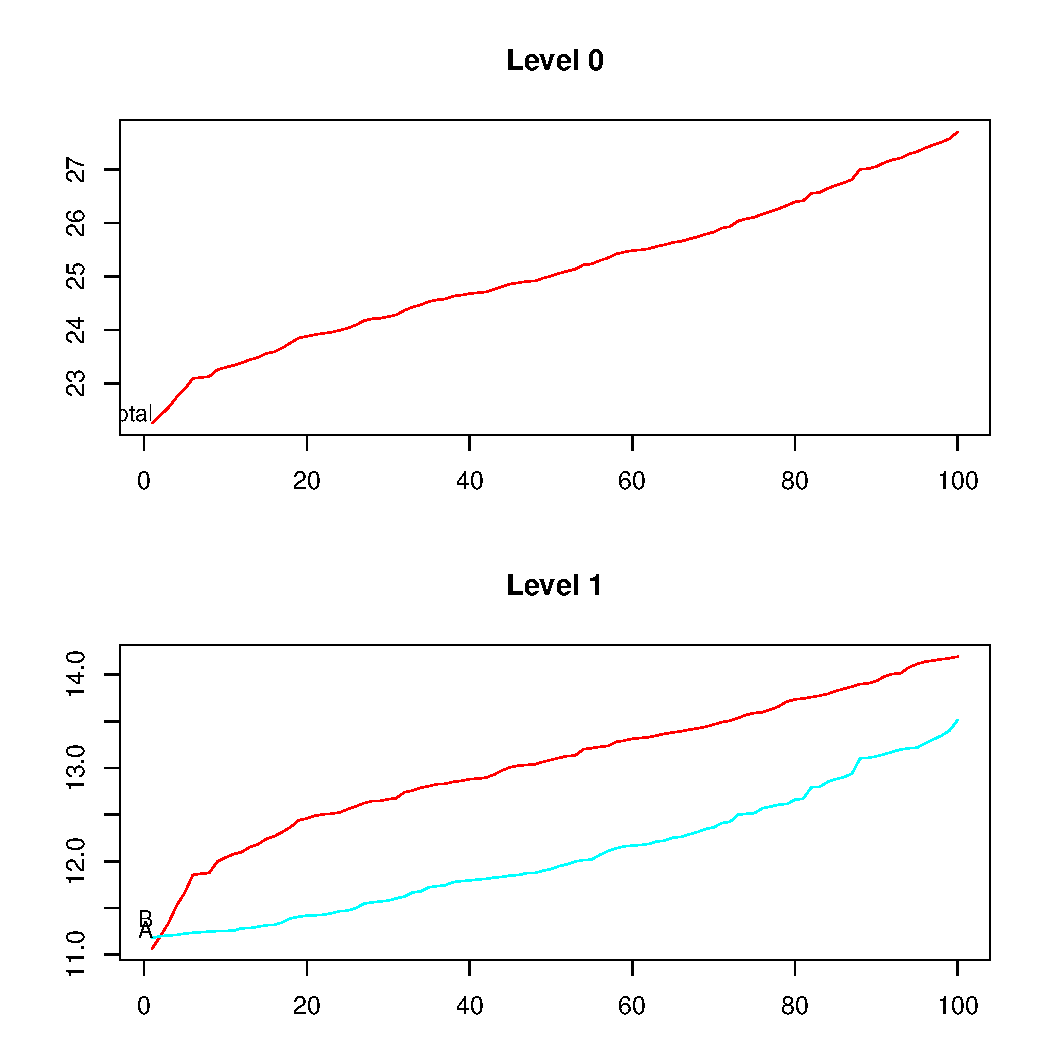
\includegraphics[width=\textwidth]{hts_plot}
\begin{Verbatim}
plot(y, levels = c(0, 1))
\end{Verbatim}
\end{figure}     

Forecasts are obtained with the \code{forecast} function. By default, it produces forecasts using the optimal combination approach with exponential smoothing (ETS) models used for the base forecasts. But other forecasting models and disaggregation methods can be specified via the following arguments:
      
\vbox{\begin{tabulary}{\linewidth}{LLL}\toprule
       fmethod && The forecasting method to be used for the base forecasts. Possible values are ``ets", ``arima" and ``rw".\\
       method && The method used for reconciling the base forecasts. It can take the following values:\\
      \end{tabulary}
   \begin{tabulary}{\linewidth}{lL}
   \hspace*{2.8cm} comb & Optimal combination forecasts; \\
   \hspace*{2.8cm} bu & Bottom-up forecasts; \\
   \hspace*{2.8cm} mo & Middle-out forecasts where the level used is specified by the level argument; \\
   \hspace*{2.8cm} tdgsa & Top-down forecasts based on the average historical proportions (Gross-Sohl method A); \\
   \hspace*{2.8cm} tdgsf  & Top-down forecasts based on the proportion of historical averages (Gross-Sohl method F);\\
   \hspace*{2.8cm} tdfp & Top-down forecasts using forecast proportions.\\
   \bottomrule
   \end{tabulary}}


\section*{Forecasting regional infant mortality counts in Australia}\label{sec:3}

We consider the infant mortality counts for eight states and territories of Australia: New South Wales (NSW), Victoria (VIC), Queensland (QLD), South Australia (SA), Western Australia (WA), Northern Territory (NT), Australian Capital Territory (ACTOT), and Tasmania (TAS). For each series, we have yearly observations on the number of infant deaths. The available data, from 1901 to 2003, were obtained from the Australian Social Science Data Archive. This data set is also publicly available in the \pkg{addb} package \citep{Hyndman10} for {\R}. Due to missing values, we use the data from 1933 to 2003 in our analysis. Based on these observations, we are interested in forecasting regional infant mortality counts from 2004 to 2013.

The data are grouped by gender and state, with two genders, eight states, and 16 series at the bottom level.

Figure~\ref{fig:3} shows the forecasts of regional infant mortality counts across Australia. The forecasts indicate a continuing decline in infant mortality counts, due to improved health services. Moreover, male mortality counts are higher than female mortality counts. Figure~\ref{fig:3} was produced using the following commands.
\begin{Verbatim}
library(hts)
# Forecast 10-step-ahead using the bottom-up method
infantforecast <- forecast(infantgts, h=10, method="bu")
# plot the forecasts including the last ten historical years
plot(infantforecast, include=10)
\end{Verbatim}
   
\begin{figure}[!htbp]
\caption{Hierarchical time-series forecasts using the bottom-up approach}\label{fig:3}
\centering
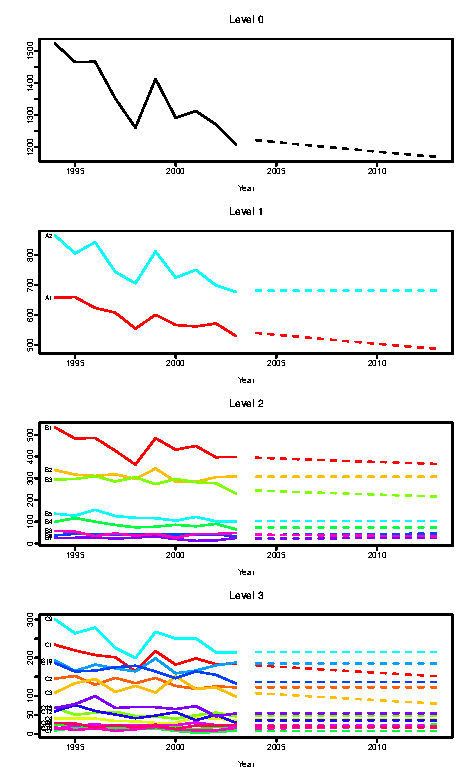
\includegraphics[width=14cm]{forecasthts}
\end{figure}

While Figure~\ref{fig:3} was produced using the \code{forecast.gts} function, there is alternative approach to produce forecasts which may give users extra flexibility.

\begin{Verbatim}
allts_infant <- aggts(infantgts)
allf <- matrix(, nrow=10, ncol=ncol(allts_infant))
# Users can select their preferred time-series forecasting method
# for each time series
for(i in 1:ncol(allts_infant))
  allf[,i] <- forecast(auto.arima(allts_infant[,i]), h=10, PI=FALSE)$mean
allf <- ts(allf, start=2004)
# combine the forecasts with the summing matrix to get a gts object
y.f <- combinef(allf, smatrix(infantgts))
\end{Verbatim}
In order to test the forecast accuracy, the \code{accuracy.gts} function can be used.
\begin{Verbatim}   # set up the training sample and testing sample
data <- window(infantgts, start=1933, end=1993)
test <- window(infantgts, start=1994, end=2003)
forecast <- forecast(data, h=10, method="bu")
# calculate ME, RMSE, MAE, MAPE, MPE and MASE
accuracy.gts(forecast, test)
\end{Verbatim}

\section*{Changes from the \pkg{hts} package version 3}
Fast computation of modeling and forecasting hierarchical and grouped time series has recently been an increasingly heated topic. Every function in the \pkg{hts} version 4 has been rewritten in order to improve its efficiency and flexibility. In addition, there are a few new features or changes made to the \pkg{hts} package.

\begin{description}
  \item[\code{hts}] Argument \code{g} is replaced with \code{nodes} implemented for the information about the hierarchical structure. The new argument \code{nodes} requires a \code{list} class containing the number of child nodes associated with the level rather than using a \code{gmatrix} concept. A hierarchy presented in the figure \ref{fig:fig-9-4-hier} suggests \code{nodes} specified as \code{list(2, c(3, 2))} referring to 2 nodes at level~1 as well as 3 and 2 nodes respectively at level~2. Apart from changes in the way of specifying the hierarchical structure, a new option \code{characters} has been added, which allows users to customize names for labelling but in a limited way. We use an example of Anatomical Therapeutic Chemical (ATC) classification system to illustrate the usage. As shown in the table \ref{tab:atc}, it's a hierarchy with six levels including level~0 and one of the bottom series is names as ``A10BA02''. In order to construct the labels according to the table \ref{tab:atc}, it can be obtained by using \code{characters = c(1, 2, 1, 1, 2)} in the \code{hts} function. \\
  \vbox{\begin{table}
    \centering
    \begin{tabulary}{\linewidth}{lL}
     \hspace*{2.8cm} A & Alimentary tract and metabolism (1st level, anatomical main group); \\
     \hspace*{2.8cm} A10 & Drugs used in diabetes (2nd level, therapeutic subgroup); \\
     \hspace*{2.8cm} A10B & Blood glucose lowering drugs, excl. insulins (3rd level, pharmacological subgroup); \\
     \hspace*{2.8cm} A10BA & Biguanides (4th level, chemical subgroup); \\
     \hspace*{2.8cm} A10BA02  & metformin (5th level, chemical substance); \\
     \bottomrule
     \end{tabulary}
     \caption{ATC classification system}
     \label{tab:atc}
   \end{table}}
 \item[\code{aggts}] The function \code{allts} is no longer available in the \pkg{hts} package; Instead, a more flexible function \code{aggts} with one more argument \code{levels} makes it possible to extract the levels of time series of interest. For instance, we are interested in observing the regional infant mortality counts across the states and they are obtained by specifying \code{levels = 2}. It's assumed to start with level~0 in all functions that have \code{levels} provided. \\
   \begin{verbatim}
    statets <- aggts(infantgts, levels = 2)  # Return time series at level 2 (State)
    plot(infantgts, levels = 2) Plot time series across the states
   \end{verbatim}
 \item[\code{forecast}] Fitted values and residuals at the bottom level are made available to users, which are reconciled in the same way as the forecasts, as long as users set \code{keep.fitted = TRUE} and \code{keep.resid = TRUE}. Furthermore, the \pkg{parallel} package has been imported for the support of parallel computing. The \code{forecast} function generates independent forecasts for each time series and it takes the substantial proportion of time to model and forecast these time series. Therefore producing forecasts in parallel enables users to save the significant amount of computing time, if \code{parallel = TRUE}. Another major change is adding a new argument \code{weights} that is associated with the optimal combination approach. It uses ordinary least squares for the unscaled forecasts in the case of \code{weights = "none"} and weighted least squares for the forecasts scaled by the standard deviation of the reconciled forecasts, when \code{weights = "sd"}. There is a special case that the bottom level series are on the same scale and the weights is equal to the inverse of the row sums of $\bm{S}$, as \code{weights = "nseries"} implemented in the \code{forecast} function. \\
   \begin{verbatim}
   fcasts <- forecast(htseg1, h = 10, method = "comb", fmethod = "arima", 
                      weights = "sd", keep.fitted = TRUE, parallel = TRUE)
   \end{verbatim}
 \item[\code{accuracy.gts}] It returns in-sample error measures at the bottom level, if \code{keep.fitted = TRUE} in the \code{forecast} function and the argument \code{test} is missing.
   \begin{verbatim}
   accuracy.gts(fcasts)  # In-sample error measure
   \end{verbatim}
\end{description}
   
\section*{Conclusion}

This article describes several techniques in the \pkg{hts} package, for modeling and forecasting hierarchical and grouped time series. The top-down approach models and forecasts time series at the top level, and then disaggregates the values based on historical or forecast proportions. The bottom-up approach models and forecasts time series at the bottom level, and then aggregates to the top level. The middle-out approach combines the top-down and bottom-up approaches. The optimal combination approach considers the problem of hierarchical forecasting from a regression perspective, and it uses ordinary least squares to find the optimal regression coefficients, from which forecasts are obtained. All hierarchical forecasting techniques described can be readily implemented in the \pkg{hts} package.

%The methods reviewed in this article focus on an ever increasing number of time series that are hierarchical in structure and clusters of which may be correlated, and the \ita{hts} package should be considered when the interest lies in modeling and forecasting the future realizations of a hierarchical/group time series.
 
\bibliography{hts}
\end{document}
%\bibliographystyle{agsm} 
  
